\portada

\begin{esquemaExplorador}
  \temaEsquema{Operadores en $\mathbb{C}^2$}{
    \conceptoEsquema{Matriz adjunta y operadores especiales}
    \conceptoEsquema{Operadores hermitianos y unitarios}
    \conceptoEsquema{Descomposición espectral}
  }
  \temaEsquema{Puertas Cuánticas de Un cúbit}{
    \conceptoEsquema{Matrices de Pauli: X, Y, Z}
    \conceptoEsquema{Puerta de Hadamard}
    \conceptoEsquema{Puertas de fase: S, T, rotaciones}
  }
  \temaEsquema{Geometría en la Esfera de Bloch}{
    \conceptoEsquema{Rotaciones como operadores unitarios}
    \conceptoEsquema{Visualización geométrica}
    \conceptoEsquema{Generación de puertas arbitrarias}
  }
  \temaEsquema{Operadores en $\mathbb{C}^n$}{
    \conceptoEsquema{Sistemas de múltiples cúbits}
    \conceptoEsquema{Operadores producto tensorial}
    \conceptoEsquema{Operadores no separables}
  }
  \temaEsquema{Puertas Cuánticas Controladas}{
    \conceptoEsquema{CNOT y puertas controladas generales}
    \conceptoEsquema{Puertas de múltiples controles}
    \conceptoEsquema{Universalidad cuántica}
  }
  \temaEsquema{Evolución Temporal y Hamiltonianos}{
    \conceptoEsquema{Operadores hermitianos como generadores}
    \conceptoEsquema{Matrices exponenciales}
    \conceptoEsquema{Simulación de evolución cuántica}
  }
\end{esquemaExplorador}

\unirsection{Ideas clave}

\subsection{Introducción y objetivos}

Habiendo establecido la teoría general de operadores lineales en el Tema 3, ahora nos enfocamos en los operadores específicos en $\mathbb{C}^2$ y $\mathbb{C}^{2^n}$ que forman el corazón de la computación cuántica. Estos operadores, cuando satisfacen la condición de unitariedad, se conocen como \textbf{puertas cuánticas} y constituyen los bloques de construcción fundamentales de los algoritmos cuánticos.

Los objetivos específicos de este tema son:

\begin{itemize}
  \item Caracterizar completamente los operadores unitarios y hermitianos en $\mathbb{C}^2$
  \item Estudiar las puertas cuánticas fundamentales y su interpretación geométrica
  \item Analizar cómo los operadores producto tensorial describen sistemas multicúbit
  \item Desarrollar puertas controladas y entender su implementación
  \item Conectar operadores hermitianos con la evolución temporal cuántica
\end{itemize}

\subsection{Operadores Especiales en $\mathbb{C}^2$}

Empecemos con el espacio de un solo cúbit, $\mathbb{C}^2$. Aquí, los operadores lineales se representan como matrices $2 \times 2$, y su estudio es fundamental para entender la computación cuántica. La dimensión del espacio de matrices $2 \times 2$ es 4, lo que implica que éste es el número de matrices linealmente independientes que cualquier base va a tener.

\begin{eje}
  Las matrices de Pauli $\{\sigma_x, \sigma_y, \sigma_z\}$ junto con la identidad es una base.

  Al coincidir el número de matrices del conjunto con la dimensión del espacio, podemos estudiar solo una condición de base, ser linealmente independiente o generar el espacio.

  Veamos que son linealmente independientes. Si existen $a, b, c, d \in \mathbb{C}$ tales que $aI + b\sigma_x + c\sigma_y + d\sigma_z = 0$, entonces
  \begin{align*}
    0 & = aI + b\sigma_x + c\sigma_y + d\sigma_z = a\begin{pmatrix} 1 & 0 \\ 0 & 1 \end{pmatrix}+b \begin{pmatrix} 0 & 1 \\ 1 & 0 \end{pmatrix}    +c \begin{pmatrix} 0 & -i \\ i & 0 \end{pmatrix}+d \begin{pmatrix} 1 & 0 \\ 0 & -1 \end{pmatrix}= \\
      & = \begin{pmatrix} a+d & b - ic \\ b + ic & a - d \end{pmatrix}\Rightarrow
    \begin{cases}
      a + d = 0  \\
      b - ic = 0 \\
      b + ic = 0 \\
      a - d = 0
    \end{cases} \Rightarrow a = b = c = d = 0\,.
  \end{align*}
\end{eje}

Cualquier matriz hermítica $H = \begin{pmatrix} a & b \\ \overline{b} & c \end{pmatrix}$ con $a, c \in \mathbb{R}$ y $b \in \mathbb{C}$ puede expresarse en esta base de la siguiente manera:
$$H = \frac{a+c}{2}I + \Rp(b)\sigma_x - \Ip(b)\sigma_y+ \frac{a-c}{2}\sigma_z $$

Es importe observar como sobre esta base, los coeficientes de la combinación lineal son reales. Por tanto, el espacio de matrices hermitianas es un espacio vectorial real de dimensión 4.

En cuanto a los operadores unitarios, la condición $U^\dagger U = I$ impone restricciones no lineales sobre los coeficientes de la combinación lineal. Por tanto, el conjunto de operadores unitarios no forma un espacio vectorial, sino un grupo bajo la multiplicación de matrices.


\begin{theo}[Parametrización de operadores unitarios]
  Todo operador unitario en $\mathbb{C}^2$ puede escribirse como:
  $$U = \begin{pmatrix} e^{i\alpha} & 0 \\ 0 & e^{i\beta} \end{pmatrix} \begin{pmatrix} \cos\frac{\theta}{2} & \sin\frac{\theta}{2} \\ -\sin\frac{\theta}{2} & \cos\frac{\theta}{2} \end{pmatrix} \begin{pmatrix} e^{-i\alpha} & 0 \\ 0 & e^{-i\beta} \end{pmatrix}$$
  donde $\alpha, \beta, \theta \in \mathbb{R}$.
\end{theo}

\begin{info}
  Debería notarse que esta parametrización no es compatible con el grupo de operadores unitarios $2 \times 2$ isomorfo a $U(2)$ y con dimensión real 4, como cabría esperar. En computación cuántica, típicamente ignoramos fases globales, y es por ello que en realidad estamos trabajando con el grupo $SU(2)/\mathbb{Z}_2 \cong SO(3)$.
\end{info}

\subsection{La esfera de Bloch}
La esfera de Bloch es una representación geométrica de los estados de un cúbit. Cada punto en la superficie de la esfera corresponde a un estado puro del cúbit, mientras que los puntos en el interior representan estados mixtos.

Todo ket $\ket{a}$ de un cúbit puede ser expresado a partir de dos valores reales, $\theta$ y $\phi$, como:
\[
  \ket{a}=\cos\left(\frac{\theta}{2}\right)\ket{0}+e^{i\phi}\sin\left(\frac{\theta}{2}\right)\ket{1}\ (\theta,\phi)\in [0, \pi]\times[0, 2\pi]
\]

\begin{figure}[H]
  \centering
  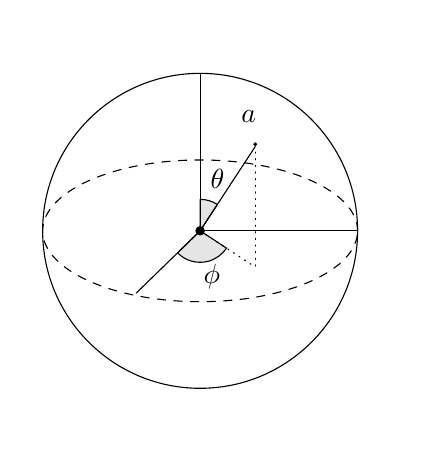
\begin{tikzpicture}
    [line cap=round, line join=round]
    \clip (-2.19,-2.49) rectangle (2.66,2.58);
    \draw [shift={(0,0)}, fill, fill opacity=0.1] (0,0) -- (56.7:0.4) arc (56.7:90.:0.4) -- cycle;
    \draw [shift={(0,0)}, fill, fill opacity=0.1] (0,0) -- (-135.7:0.4) arc (-135.7:-33.2:0.4) -- cycle;
    \draw (0,0) circle (2cm);
    \draw [rotate around={0.:(0.,0.)},dash pattern=on 3pt off 3pt] (0,0) ellipse (2cm and 0.9cm);
    \draw (0,0)-- (0.70,1.07);
    \draw (0,0) -- (0,2);
    \draw (0,0) -- (-0.81,-0.79);
    \draw (0,0) -- (2,0);
    \draw [dotted] (0.7,1) -- (0.7,-0.46);
    \draw [dotted] (0,0) -- (0.7,-0.46);
    \draw (-0.08,-0.3) node[anchor=north west] {$\phi$};
    \draw (0.01,0.9) node[anchor=north west] {$\theta$};
    \draw (0.4,1.65) node[anchor=north west] {$\ket{a}$};
    \scriptsize
    \draw [fill] (0,0) circle (1.5pt);
    \draw [fill] (0.7,1.1) circle (0.5pt);
  \end{tikzpicture}
  \caption{Representación de un ket $\ket{a}\in\H$ en la esfera de Bloch}
\end{figure}

Por convenio, se dibuja la esfera sobre los tres ejes espaciales X, Y, Z de tal modo que el ecuador quede en el plano XY, igualmente se considera el eje Z perpendicular a dicho plano.
Los kets de la base canónica computacional se sitúan sobre el eje Z, estando el ket $\ket{0}$ en el eje positivo y el ket $\ket{1}$ sobre el eje negativo.

\begin{figure}[H]
  \centering
  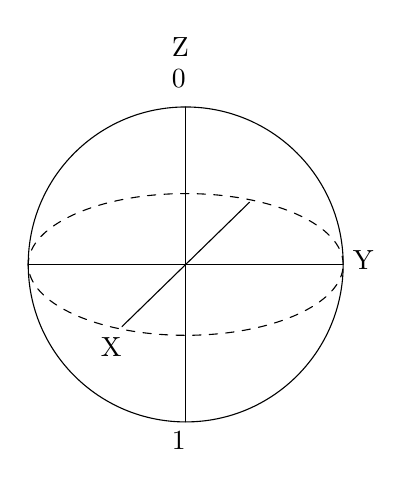
\begin{tikzpicture}
    [line cap=round, line join=round]
    \draw (0,0) circle (2cm);
    \draw [rotate around={0.:(0.,0.)},dash pattern=on 3pt off 3pt] (0,0) ellipse (2cm and 0.9cm);
    \draw (0,0) -- (0,2);
    \draw (0,0) -- (0,-2);
    \draw (0,0) -- (2,0);
    \draw (0,0) -- (-2,0);
    \draw (0,0) -- (-0.81,-0.79);
    \draw (0,0) -- (0.81,0.79);
    \draw (-0.3,3) node[anchor=north west] {Z};
    \draw (-0.3,2.6) node[anchor=north west] {$\ket{0}$};
    \draw (-0.3,-2) node[anchor=north west] {$\ket{1}$};
    \draw (2,0.3) node[anchor=north west] {Y};
    \draw (-1.2,-0.8) node[anchor=north west] {X};
  \end{tikzpicture}
  \caption{Ejes espaciales y representación de la base canónica computacional en la esfera de Bloch}
\end{figure}

\begin{eje}
  Así por ejemplo, el estado $\ket{+} = \frac{1}{\sqrt{2}}(\ket{0} + \ket{1})$ es imagen del ket $\ket{0}$ al aplicar la puerta de Hadamard, y corresponde al punto en el ecuador con $\phi=0$.

  Esta representación geométrica permite visualizar la puerta de Hadamard como una rotación de $90°$ alrededor del eje Y.

  Mientras que $\ket{-} = \frac{1}{\sqrt{2}}(\ket{0} - \ket{1})$ corresponde al punto en el ecuador con $\phi=\pi$.
\end{eje}

\begin{info}
  La esfera de Bloch proporciona una visualización intuitiva de las operaciones cuánticas como rotaciones en el espacio tridimensional. Cada operador unitario en $\mathbb{C}^2$ corresponde a una rotación de la esfera.
\end{info}

\subsection{Puertas Cuánticas Fundamentales de un cúbit}

Ya hemos que las matrices de Pauli son las puertas cuánticas más fundamentales y corresponden con rotaciones de $\pi/2$ alrededor de los ejes de la esfera de Bloch. Como puertas dentro del contexto de la computación cuántica, se suelen denotar por las letras $X, Y, Z$ en lugar de $\sigma_x, \sigma_y, \sigma_z$.

\begin{defi}[Puertas de Pauli]
  \begin{align*}
    X & = \sigma_x = \begin{pmatrix} 0 & 1 \\ 1 & 0 \end{pmatrix} \quad \text{(puerta NOT)}      \\
    Y & = \sigma_y = \begin{pmatrix} 0 & -i \\ i & 0 \end{pmatrix}                               \\
    Z & = \sigma_z = \begin{pmatrix} 1 & 0 \\ 0 & -1 \end{pmatrix} \quad \text{(puerta de fase)}
  \end{align*}
\end{defi}

\subsubsection{Puerta de Hadamard}

\begin{defi}[Puerta de Hadamard]
  $$H = \frac{1}{\sqrt{2}}\begin{pmatrix} 1 & 1 \\ 1 & -1 \end{pmatrix}$$
\end{defi}

La puerta de Hadamard es fundamental para crear superposiciones, y su acción sobre los estados de la base computacional es:
\begin{itemize}
  \item $H\ket{0} = \ket{+} = \frac{1}{\sqrt{2}}(\ket{0} + \ket{1})$.
  \item $H\ket{1} = \ket{-} = \frac{1}{\sqrt{2}}(\ket{0} - \ket{1})$.
\end{itemize}

Las siguientes identidades conectan las puertas de Pauli y la puerta de Hadamard:
\begin{align*}
  HXH & = Z  \\
  HZH & = X  \\
  HYH & = -Y
\end{align*}

\subsubsection{Puertas de fase}

\begin{defi}[Puertas de fase]
  \begin{align*}
    R_\phi & = \begin{pmatrix} 1 & 0 \\ 0 & e^{i\phi} \end{pmatrix} \quad \text{(puerta de fase general)} \\
    S      & = \begin{pmatrix} 1 & 0 \\ 0 & i \end{pmatrix} = R_{\frac{\pi}{2}}                           \\
    T      & = \begin{pmatrix} 1 & 0 \\ 0 & e^{i\pi/4} \end{pmatrix} = R_{\frac{\pi}{4}}
  \end{align*}
\end{defi}

Las puertas de fase introducen una fase relativa entre los estados $\ket{0}$ y $\ket{1}$, y son cruciales para muchos algoritmos cuánticos. Estas puertas se relacionan entre sí mediante las siguientes identidades:
\begin{itemize}
  \item $S^2 = Z$
  \item $T^2 = S$
  \item $T^4 = Z$
  \item $T^8 = I$
\end{itemize}

\subsection{Rotaciones en la Esfera de Bloch}

Toda rotación en la esfera de Bloch corresponde a un operador unitario en $\mathbb{C}^2$:

\begin{defi}[Rotaciones de Pauli]
  Las rotaciones alrededor de los ejes de Pauli son:
  \begin{align*}
    R_x(\theta) & = e^{-i\theta\sigma_x/2} = \cos\frac{\theta}{2}I - i\sin\frac{\theta}{2}\sigma_x = \begin{pmatrix} \cos\frac{\theta}{2} & -i\sin\frac{\theta}{2} \\ -i\sin\frac{\theta}{2} & \cos\frac{\theta}{2} \end{pmatrix} \\
    R_y(\theta) & = e^{-i\theta\sigma_y/2} = \cos\frac{\theta}{2}I - i\sin\frac{\theta}{2}\sigma_y = \begin{pmatrix} \cos\frac{\theta}{2} & -\sin\frac{\theta}{2} \\ \sin\frac{\theta}{2} & \cos\frac{\theta}{2} \end{pmatrix}    \\
    R_z(\theta) & = e^{-i\theta\sigma_z/2} = \cos\frac{\theta}{2}I - i\sin\frac{\theta}{2}\sigma_z = \begin{pmatrix} e^{-i\theta/2} & 0 \\ 0 & e^{i\theta/2} \end{pmatrix}
  \end{align*}
\end{defi}

\begin{theo}[Descomposición universal para $SU(2)$]
  Toda matriz unitaria $U \in SU(2)$ puede descomponerse como:
  $$U = e^{i\alpha}R_z(\beta)R_y(\gamma)R_z(\delta)$$
  para algunos ángulos reales $\alpha, \beta, \gamma, \delta$.
\end{theo}

\begin{eje}[Implementación de rotación arbitraria]
  Para implementar una rotación alrededor del vector $\hat{n} = (n_x, n_y, n_z)$ por ángulo $\theta$:
  $$R_{\hat{n}}(\theta) = \cos\frac{\theta}{2}I - i\sin\frac{\theta}{2}(n_x\sigma_x + n_y\sigma_y + n_z\sigma_z)$$
\end{eje}

\subsection{Operadores en $\mathbb{C}^n$: Sistemas multicúbit}

Recordemos que el espacio de estados de un sistema de $n$ cúbits es el producto tensorial de $n$ copias de $\mathbb{C}^2$ y tiene dimensión $2^n$, y por construcción de la base computacional, la base canónica de $\mathbb{C}^{2^n}$ es:

$$\{\ket{b_1 b_2 \ldots b_n} : b_i \in \{0,1\}\}$$

\begin{eje}[Sistema de 2 cúbits]
  Para $n = 2$, tenemos $\mathbb{C}^4$ con base $\{\ket{00}, \ket{01}, \ket{10}, \ket{11}\}$:
  $$\ket{00} = \begin{pmatrix} 1 \\ 0 \\ 0 \\ 0 \end{pmatrix}, \quad \ket{01} = \begin{pmatrix} 0 \\ 1 \\ 0 \\ 0 \end{pmatrix}, \quad \ket{10} = \begin{pmatrix} 0 \\ 0 \\ 1 \\ 0 \end{pmatrix}, \quad \ket{11} = \begin{pmatrix} 0 \\ 0 \\ 0 \\ 1 \end{pmatrix}$$
\end{eje}

Mientras que la operación tensorial se construye a partir de la base canónica, los operadores en sistemas multicúbit pueden ser más complejos.
Si $A$ actúa sobre el cúbit $i$ y $B$ actúa sobre el cúbit $j$, entonces:
$$(A \otimes B)(\ket{ij}) = (A \otimes B)(\ket{i} \otimes \ket{j}) = (A\ket{i}) \otimes (B\ket{j})= \ket{AiBj}$$

\begin{eje}[Aplicación de operadores producto]
  $$(X \otimes I)\ket{01} = X\ket{0} \otimes I\ket{1} = \ket{1} \otimes \ket{1} = \ket{11}$$
  $$(I \otimes Z)\ket{10} = I\ket{1} \otimes Z\ket{0} = \ket{1} \otimes \ket{0} = \ket{10}$$
\end{eje}

\subsubsection{La puerta CNOT}

\begin{defi}[Puerta CNOT]
  La puerta Controlled-NOT actúa sobre dos cúbits:
  $$\text{CNOT} = \begin{pmatrix} 1 & 0 & 0 & 0 \\ 0 & 1 & 0 & 0 \\ 0 & 0 & 0 & 1 \\ 0 & 0 & 1 & 0 \end{pmatrix}$$

  Equivalentemente:
  $$\text{CNOT} = \ket{0}\bra{0} \otimes I + \ket{1}\bra{1} \otimes X$$
\end{defi}

\begin{eje}[Acción de CNOT]
  \begin{align*}
    \text{CNOT}\ket{00} & = \ket{00} \\
    \text{CNOT}\ket{01} & = \ket{01} \\
    \text{CNOT}\ket{10} & = \ket{11} \\
    \text{CNOT}\ket{11} & = \ket{10}
  \end{align*}

  El primer cúbit actúa como control: si está en $\ket{1}$, se aplica $X$ al segundo cúbit.
\end{eje}

\subsubsection{Puertas controladas generales}

\begin{defi}[Puerta controlada general]
  Para cualquier operador unitario $U$ de un cúbit:
  $$C_U = \ket{0}\bra{0} \otimes I + \ket{1}\bra{1} \otimes U = \begin{pmatrix} I & 0 \\ 0 & U \end{pmatrix}$$
\end{defi}

\begin{eje}[Otras puertas controladas importantes]
  \begin{itemize}
    \item \textbf{Controlled-Z}: $C_Z = \text{diag}(1, 1, 1, -1)$
    \item \textbf{Controlled-Hadamard}: $C_H = \begin{pmatrix} I & 0 \\ 0 & H \end{pmatrix}$
    \item \textbf{Controlled-Phase}: $C_{R_\phi} = \text{diag}(1, 1, 1, e^{i\phi})$
  \end{itemize}
\end{eje}

\subsubsection{Puertas de múltiples controles}

\begin{defi}[Puerta Toffoli (CCNOT)]
  La puerta Toffoli es un CNOT con dos controles:
  $$\text{CCNOT} = \text{diag}(1, 1, 1, 1, 1, 1, 0, 0) + \text{diag}(0, 0, 0, 0, 0, 0, 1, 1) \cdot \text{SWAP}_{67}$$

  Aplica $X$ al tercer cúbit solo si los primeros dos están en $\ket{11}$.
\end{defi}

\subsection{Evolución Temporal y Hamiltonianos}

\subsubsection{Operadores hermitianos como generadores}

\begin{theo}[Ecuación de Schrödinger para sistemas finitos]
  La evolución temporal de un sistema cuántico cerrado está gobernada por:
  $$\frac{d}{dt}\ket{\psi(t)} = -\frac{i}{\hbar}H\ket{\psi(t)}$$
  donde $H$ es el Hamiltoniano (operador hermitiano).
\end{theo}

La solución formal es:
$$\ket{\psi(t)} = e^{-iHt/\hbar}\ket{\psi(0)}$$

\begin{eje}[Evolución bajo Hamiltoniano de Pauli]
  Para $H = \omega\sigma_z/2$:
  $$e^{-iHt} = e^{-i\omega t\sigma_z/2} = \cos\frac{\omega t}{2}I - i\sin\frac{\omega t}{2}\sigma_z = \begin{pmatrix} e^{-i\omega t/2} & 0 \\ 0 & e^{i\omega t/2} \end{pmatrix}$$

  Un cúbit inicialmente en $\ket{+}$ evoluciona como:
  $$\ket{\psi(t)} = \frac{1}{\sqrt{2}}(e^{-i\omega t/2}\ket{0} + e^{i\omega t/2}\ket{1})$$
\end{eje}

\subsubsection{Matrices exponenciales}

\begin{theo}[Cálculo de matrices exponenciales]
  Para una matriz hermitiana $H$ con descomposición espectral $H = \sum_i \lambda_i P_i$:
  $$e^{-iHt} = \sum_i e^{-i\lambda_i t} P_i$$
  donde $P_i$ son las proyecciones sobre los subespacios propios.
\end{theo}

\begin{eje}[Exponencial de combinaciones de Pauli]
  Para $H = \alpha\sigma_x + \beta\sigma_y + \gamma\sigma_z$ con $|\vec{n}| = \sqrt{\alpha^2 + \beta^2 + \gamma^2}$:
  $$e^{-iHt} = \cos(|\vec{n}|t)I - i\sin(|\vec{n}|t)\frac{\vec{n} \cdot \vec{\sigma}}{|\vec{n}|}$$
\end{eje}

\begin{theo}
  Cualquier operador unitario en $\mathbb{C}^{2^n}$ puede aproximarse arbitrariamente bien usando solo las puertas $H$, $T$, y CNOT.
\end{theo}

\begin{info}
  Este resultado es fundamental para la computación cuántica práctica, ya que muestra que solo necesitamos implementar físicamente un pequeño conjunto de puertas para realizar cualquier cálculo cuántico.
\end{info}
